\documentclass[tikz,border=6pt]{standalone}
\usepackage{amsmath}
\usepackage{xcolor}

\definecolor{blockblue}{HTML}{4A90D9}

\begin{document}
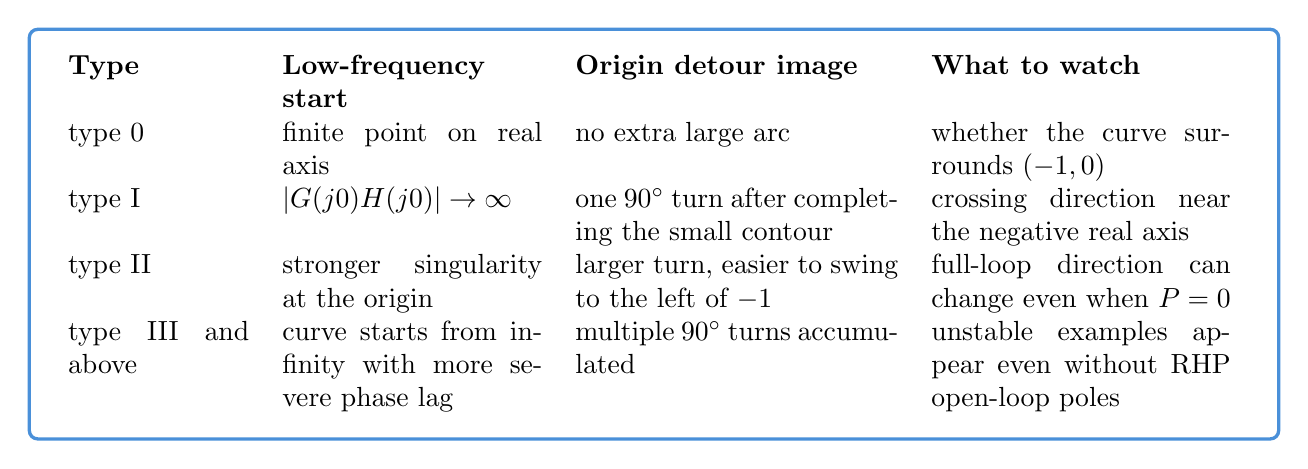
\begin{tikzpicture}[line width=1.2pt]
  \node[
    draw=blockblue,
    rounded corners=3pt,
    inner sep=8pt,
    align=left
  ] at (0,0) {
    \begin{tabular}{p{2.3cm}p{3.3cm}p{4.1cm}p{3.8cm}}
      \textbf{Type} & \textbf{Low-frequency start} & \textbf{Origin detour image} & \textbf{What to watch} \\
      type 0 & finite point on real axis & no extra large arc & whether the curve surrounds $(-1,0)$ \\
      type I & $|G(j0)H(j0)|\to\infty$ & one $90^\circ$ turn after completing the small contour & crossing direction near the negative real axis \\
      type II & stronger singularity at the origin & larger turn, easier to swing to the left of $-1$ & full-loop direction can change even when $P=0$ \\
      type III and above & curve starts from infinity with more severe phase lag & multiple $90^\circ$ turns accumulated & unstable examples appear even without RHP open-loop poles \\
    \end{tabular}
  };
\end{tikzpicture}
\end{document}
